\section{Apresentação dos Problemas}

Como a prova apresentada nesse artigo utiliza um framework, ela pode se
tornar um pouco abstrata demais. Nessa sessão apresentamos os problemas envolvidos e exemplos de cada um.

\subsection{The Legend of Zelda: a Link to The Past}

The Legend of Zelda: a Link to The Past é um jogo desenvolvido para Super Nintendo 
(que a partir desse momento será chamado apenas de Zelda, para facilitar a leitura), publicado pela
primeira vez em 1991, no Japão. Nele, controlamos o protagonista Link, um garoto que tem como objetivo
salvar a terra de Hyrule, impedir que o mago Ganon se torne o novo governante e salvar a princesa Zelda.
Para isso, Link deve obter a Triforce, uma relíquia sagrada espalhada pelo mapa, que é composta por 
três triângulos equiláteros, que trazem ao portador sabedoria, coragem e poder.

Em termos de design, o jogo é um mapa aberto, em que o jogador pode andar livremente. A câmera é posicionada acima
do plano, dando visão de uma parte do mapa total, sendo que quando o jogador se desloca para fora desse enquadramento
a câmera se desloca para exibir uma nova parte do mapa. O jogo é uma mistura de combates e puzzles. Para avançar
no jogo, é preciso explorar cavernas e construções, conversar com personagens e derrotar inimigos, assim obtendo
novos itens e habilidades. Os itens podem ser achados dentro de baús, sendo que existem itens especiais que quando são
encontrados seus baús permanecem abertos. Itens comuns podem voltam a ter seus baús fechados quando o jogador se move para
outro pedaço do mapa e retorna ao pedaço original (inimigos têm o mesmo comportamento, ou seja, a não ser que sejam chefes
especiais, os inimigos retornam ao mapa após morrerem caso haja essa troca de tela. Chefes especiais também liberam itens especiais).
Como Zelda é um jogo de mapa aberto, qualquer inimigo pode ser enfrentado a qualquer momento, desde que seja possível chegar até ele, dando grande liberdade ao jogador.

Tais itens e habilidades não são em si importantes para a prova que iremos realizar,
mas certamente poderiam ser utilizados para provar a NP-Completude por outros caminhos, como por exemplo realizando
uma redução ao problema 1-Push 2D \cite{demaine2000pushpush}.

\begin{figure}[!htb]
     \centering
     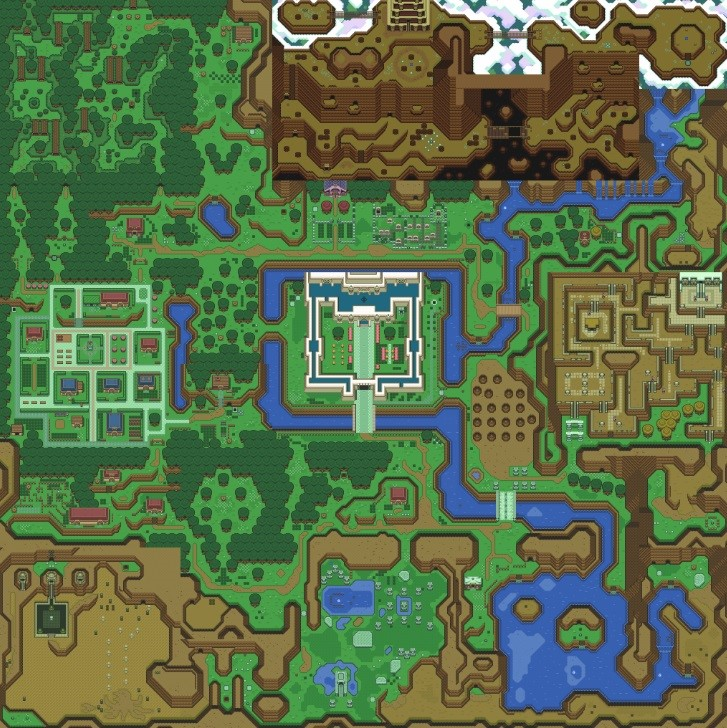
\includegraphics[scale=0.3]{zelda.jpg}
     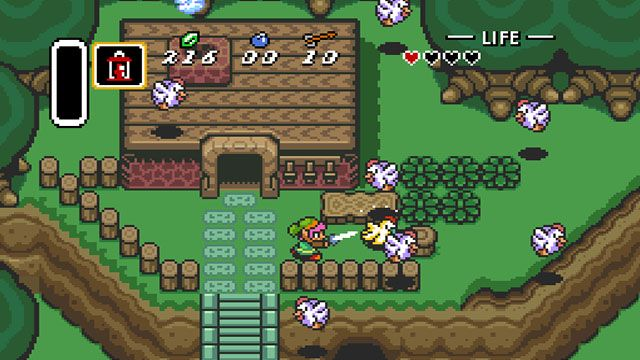
\includegraphics[scale=0.3]{link.jpg}
     \caption{Imagens do jogo}
\end{figure}

Diversos elementos do jogo podem ser utilizados para provar sua NP-Completude. Nesse jogo específico da franquia existe
um elemento bastante importante para esta prova, que o diferencia de seus anteriores: um gancho que Link pode utilizar
para se mover em direção a qualquer bloco do cenário.

\begin{figure}[!htb]
     \centering
     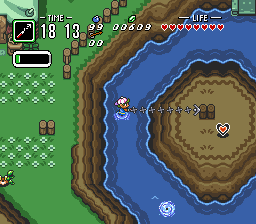
\includegraphics[scale=0.8]{hookshot.png}
     \caption{Exemplo de uso do gancho}
\end{figure}

\subsection{3-SAT}

O problema de satisfazibilidade booleana (SAT) é um problema de decisão, cuja instancia é uma escrita com operadores lógicos AND, OR, NOT, variáveis, e parênteses. A questão desse problema de decisão é: dada uma expressão, há alguma atribuição de valores verdadeiros e falsos para as variáveis que torne toda a expressão verdadeira? Uma fórmula da lógica proposicional é dita satisfazível se e somente se é possível atribuir valores lógicos a suas variáveis de tal maneira que eles tornem a fórmula verdadeira. A prova da NP Completude do problema SAT é dada pelo teorema de Cook-Levin \cite{cook1971complexity}.

O problema 3-SAT é um subconjunto do problema SAT, onde cada expressão lógica terá apenas três literais.

\begin{figure}[!htb]
     \centering
     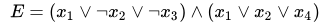
\includegraphics[scale=0.8]{cook.png}
     \caption{Exemplo do problema 3-SAT}
\end{figure}